\section{Experiments}
\label{sec:experiments}
% \tk{order: CLEVR + baselines without TL, COG + baseline without TL, Feature Transfer-CLEVR/CoGenT, Temporal Transfer - COG, Reasoning Transfer - CLEVR/CoGenT, Reasoning Transfer-COG}

We implemented and trained our SAMNet model using MI-Prometheus~\cite{kornuta2018accelerating}, a framework based on PyTorch~\cite{paszke2017automatic}.
We evaluated the model on 
the CLEVR dataset~\cite{johnson2017clevr}, a diagnostic dataset for Image Question Answering and on the COG dataset~\cite{yang2018dataset}, a video reasoning~\cite{mogadala2019trends} dataset developed for the purpose of research on relational and temporal reasoning.
We briefly describe both datasets in the following two subsections.
We also present comparison of SAMNet with the existing baselines as a sanity check. 
In all experiments we used SAMNet using $k = 8$ reasoning steps and external memory with $N = 8$ slots, each storing an array of 128 floats. 

The rest of experiments is following the proposed taxonomy.
First, we investigate the feature transfer using the CLEVR-CoGenT variants, followed by the temporal transfer on COG. Finally, we assess SAMNet's transfer reasoning capabilities on both datasets by regrouping and reorganizing classes of questions into new training and test splits.

\begin{table}[b!]
	\centering
	%\begin{adjustbox}{width=0.45\textwidth}
	\begin{tabular}{cccc}
		\toprule
		Variant	& Cubes	& Cylinders &	Spheres	\\
		\midrule
		CLEVR &  Any Color  & Any Color 	&	Any color  \\
		CoGenT-A &  Family A  & Family B 	&	Any color  \\
		CoGenT-B	&	Family B  &	Family A	&	Any color \\
		\bottomrule
	\end{tabular}
	%\end{adjustbox}
	\caption{Allowed feature combinations in the CoGenT-A and CoGenT-B variants of the CLEVR dataset.}%\vspace{2pts}
	\label{tab:cogent_conditions}
\end{table}

\begin{figure*}[t!]
	\centering
	\begin{subfigure}{\textwidth}
		\centering
		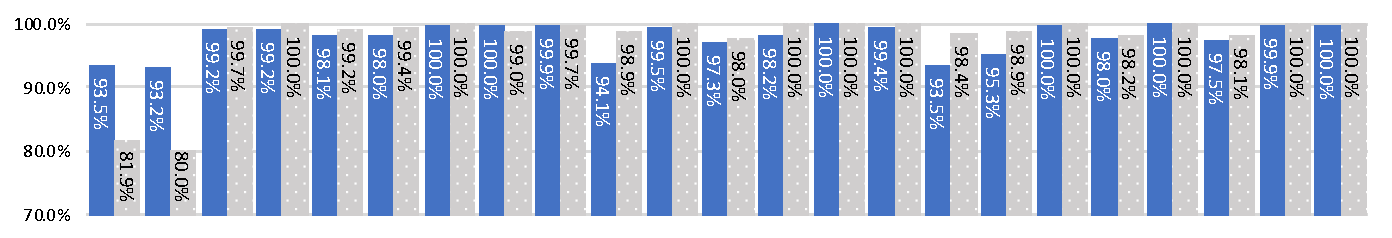
\includegraphics[width=0.9\textwidth]{../img/plots/cog_canonical_baseline_no_labels.pdf}
	\end{subfigure}%
	\newline
	\begin{subfigure}{\textwidth}
		\centering
		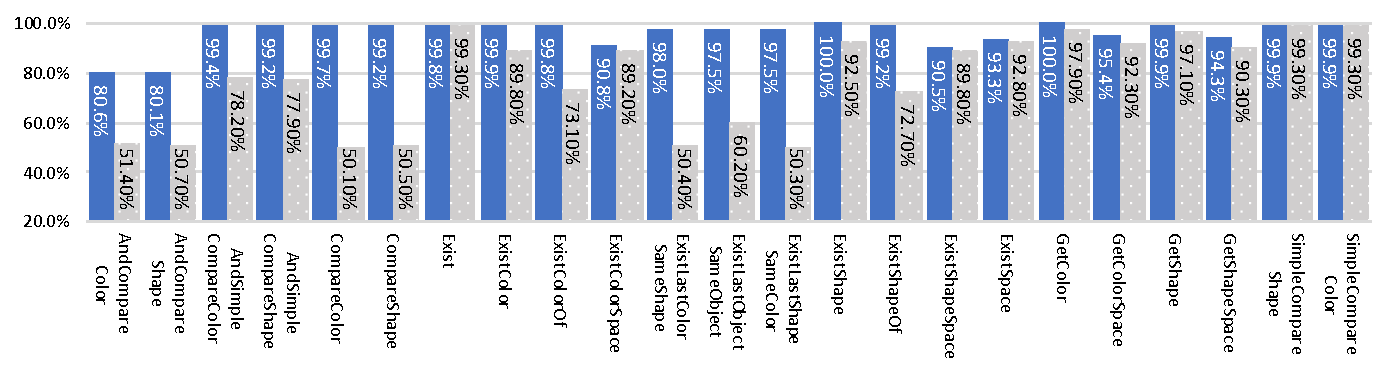
\includegraphics[width=0.9\textwidth]{../img/plots/cog_hard_baseline_labels.pdf}
	\end{subfigure}%
	\caption{Comparison of test set accuracies of SAMNet (blue) with original results achieved by the baseline model~\cite{yang2018dataset} (dotted gray) on Canonical (top) and Hard (bottom) variants of the COG dataset.}
	\label{fig:samnet_cog_detailed}
\end{figure*}

\subsection{Basic performance of SAMNet on CLEVR}
\label{sec:clevr-baseline-compare}
CLEVR images contain objects characterised by a set of simple atributes (shape, color, size and material), whereas questions are grouped into 5 categories: \textit{Exist}, \textit{Count}, \textit{CompareInteger}, \textit{CompareAttribute}, \textit{QueryAttribute}.
Along with CLEVR the authors also introduced two CLEVR-CoGenT (Constrained Generalization Test) variants, with varying combinations of color-shape attributes.
The colors are partitioned into two complementary families:
Gray, Blue, Brown and Yellow in Family A; and Red, Green, Purple, Cyan in Family B.
The cubes and cylinders take colors from complementary families in each variant with opposite configurations; the spheres can take any color in both varianrs (See~\cref{tab:cogent_conditions}).
As the input domain consist of the set of objects with all attribute values, both variants differ by their marginal distributions $P_S$ and $P_T$.

\begin{figure}[htbp]
	\centering
	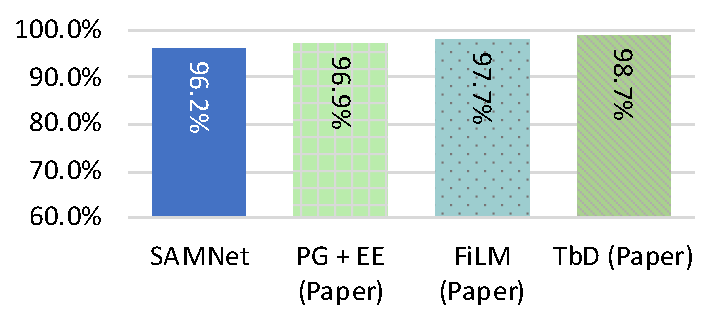
\includegraphics[width=0.8\columnwidth]{../img/plots/clevr_baselines.pdf}
	\caption{Comparison of SAMNet to baselines on CLEVR.}
	\label{fig:clevr_baselines}
\end{figure}


We compare SAMNet's performance to selected SOTA models, namely Transparency by Design networks (TbD)~\cite{mascharka2018transparency}, Feature-wise Linear Modulation (FiLM)~\cite{perez2018film} and the Program Generator + Execution Engine (PG + EE)~\cite{johnson2017inferring}.
For performance reasons, we deactivated the external memory and temporal-related modules in SAMNet as they are unnecessary while reasoning about static images.
As presented in \cref{fig:clevr_baselines}, SAMNet reaches comparable 96.2\% accuracy, compared to 96.9\%, 97.7\% and 98.7\% for PG + EE, FiLM and TbD respectively.


\subsection{Basic performance of SAMNet on COG}
\label{sec:cog-baseline-compare}

GOC dataset contains short videos with the associated questions, grouped into 23 question categories~\footnote{Aside of categorical questions, COG also offers tasks expecting the model to point a particular object in the image (out of scope of this paper).}.
COG comes in two variants: the Canonical (easy) and Hard, differing mainly on the number of frames in the video, the maximum amount of look-back in frame history containing relevant information for reasoning, and the number of object distractors (see~\cref{tab:cog_variants}).
Since the number of task classes is large, we designed a 2-level hierarchy of task groups using the
description of tasks, as shown in~\cref{fig:task-groups}.

\begin{table}[ht]
	\centering
	\begin{tabular}{lccc}
		\toprule
		Variant	& Frames & History	& Distractors \\
		\midrule
		Canonical (Easy) & 4 & 3 & 1\\
		Hard  & 8 & 7 & 10\\
		\bottomrule
	\end{tabular}
	\caption{Details of the Canonical and Hard variants of COG.}
	\label{tab:cog_variants}
\end{table}


\begin{figure}[htbp]
	\centering
	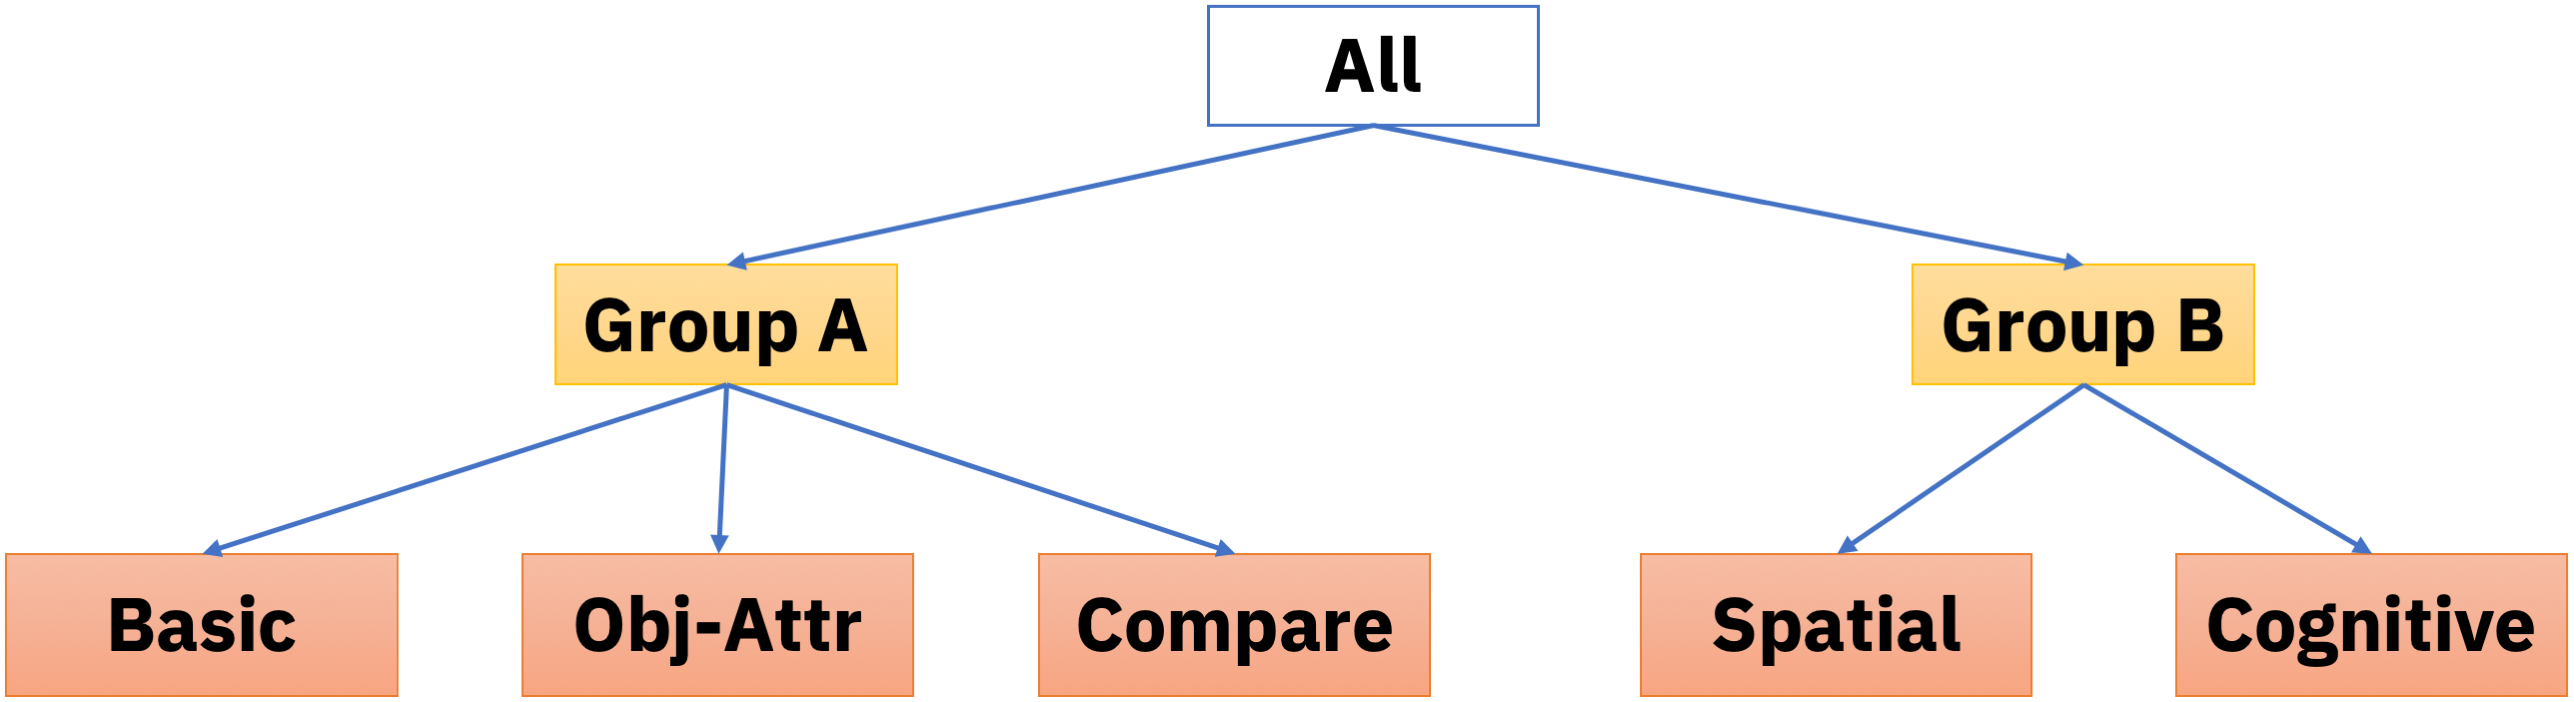
\includegraphics[width=\columnwidth]{../img/architecture/hierarchy}
	\caption{Hierarchy of Task Groups in the COG dataset.}
	\label{fig:task-groups}
\end{figure}



For groups at the lowest level, we chose the following task classes to be placed in those groups.
Below, substitute each of \textit{Shape} and \textit{Color} for  \uX{} to obtain the task class.
\begin{description}
	\compresslist
	\item[Basic:] \textit{Exist}\uX, \textit{Get}\uX{} and \textit{Exist};
	\item[Obj-Attr:] \emph{SimpleCompare}\uX{} and \textit{AndSimpleCompare}\uX;
	\item[Compare:] \textit{Compare}\uX,  \textit{AndCompare}\uX{} \& \textit{Exist}\uX\textit{Of};
	\item[Spatial:] \textit{ExistSpace}, \textit{Exist}\uX\textit{Space}, and \textit{Get}\uX\textit{Space};
	\item[Cognitive:] \textit{ExistLastColorSameShape}, \textit{ExistLastShapeSameColor} and \textit{ExistLastObjectSameObject}
\end{description}


We compared our results with the baseline model introduced in the same paper as the COG dataset~\cite{yang2018dataset}.
The most important results are highlighted in~\cref{fig:samnet_cog_detailed}; full comparison can be found in the supplementary material.

For the Canonical variant (top row), we achieve similar accuracies for the majority of tasks (with a total average accuracy of 98.0\%, compared to 97.6\% for the baseline model), with significant improvements (around 13 points) for \textit{AndCompare} tasks.
As these tasks focus on compositional questions referring to two objects, we hypothesize that our model achieves better accuracy due to its ability to selectively pick and store relevant objects from the past frames in its external memory.
For the Hard variant, we achieve a total average accuracy of 96.1\% compared to 80.1\% for the baseline model, demonstrating that our model can adapt to larger number of frames and distractors.
SAMNet improves upon the baseline model on all tasks, with improvements varying from 0.5 to more than 30 points, shining in the most complex (\textit{AndCompare}\uX, \textit{Compare}\uX) tasks.


\subsection{Feature transfer using CLEVR-CoGenT}
\label{sec:feature}

In order to quantify SAMNet feature transfer capabilities we used the CoGenT variants of CLEVR and performed set of experiments, starting from training on CoGenT-A followed by:
an immediate test (zero-shot learning) to test split ot CoGenT-B; and fine-tuning for a single epoch on 30k samples from CoGenT-B before testing (following methodology used in~\cite{johnson2017inferring, mascharka2018transparency, perez2018film, marois2018transfer}).
In \cref{fig:CoGenT-B-results} we compare the achieved performance with the previously selected SOTA models. 
As sanity check we also provide accuracies achieved when: tested directly on CoGenT-A; and tested on CoGenT-A after fine-tuning on B.

\begin{figure}[htbp]
	\centering
	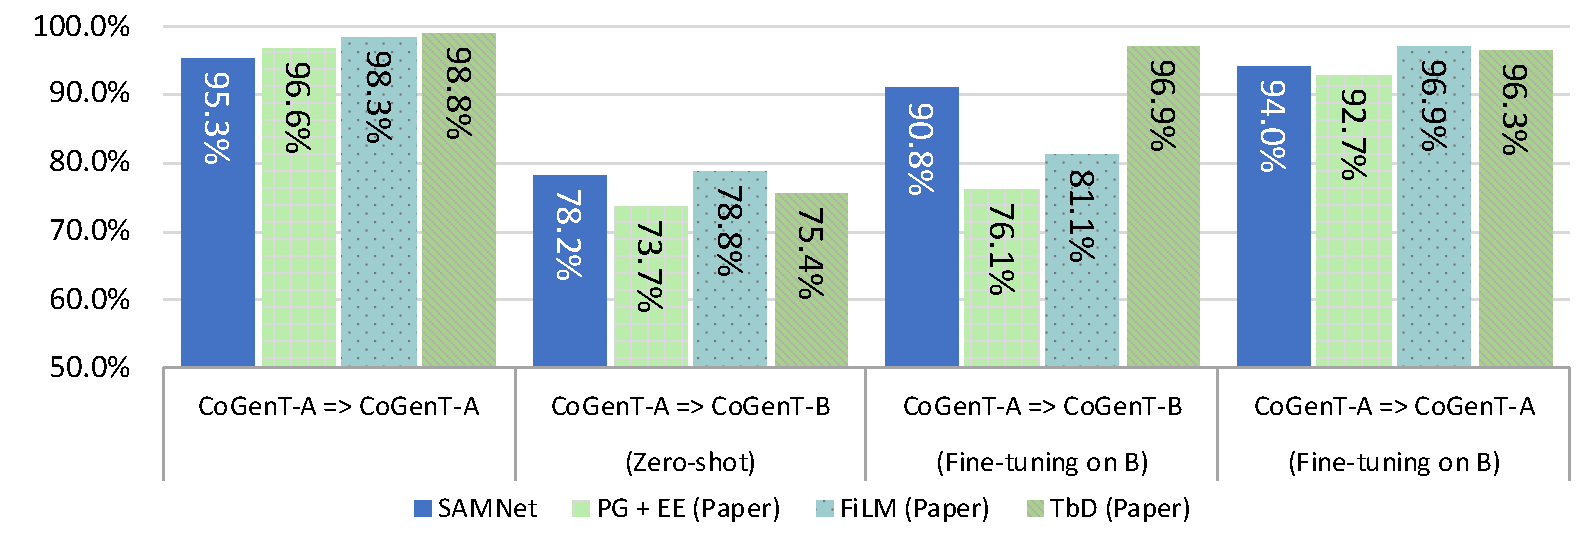
\includegraphics[width=\columnwidth]{../img/plots/cogent_feature_transfer_baselines.pdf}
	\caption{Test accuracy on CoGenT-A \& -B when training on CoGenT-A and fine-tuning on CoGenT-B.}
	\label{fig:CoGenT-B-results}
\end{figure}

When training and testing on CoGenT-A, SAMNet performs slightly worse than the other models.
In the case of zero-shot transfer to CoGenT-B all models show relatively good performance (around 75 percent), still being a significant decrease of accuracy (by 17 points)
As expected, all models are able to recove performance when fine-tuned on CoGenT-B.
This process results in degradation of performance on originallly mastered CoGenT-A, with SAMNet and TbD showing clear capabilities to limit the impact of catastrophic forgetting.
This indicates that both SAMNet and TbD managed to develop and sustain (to some extent) representations of features when facing shift from one domain to the other.
Still, the drop in zero-shot transfer suggests that both struggle with disentanglement of shape and color features.

\subsection{Temporal transfer in COG}
\label{sec:temporal}

The goal here is to test the transfer learning ability concerning the frame sequence length, frame history required for reasoning, and the number of object distractors.
For that purpose, we compare both models when trained on the Canonical variant but tested on the Hard variant (\cref{fig:samnet_cog_overall_transfer}).
The gray (dotted) color indicates original accuracies of the baseline model from paper,
whereas yellow (striped) indicates accuracies of the baseline model obtained by running the original code provided by the authors~\cite{yang2018implement}.

The first column displays the scores of the traditional ML setup when training and testing on the Canonical variant.
The observed close scores in gray (dotted) and yellow (striped) underscore the baseline model reproducibility.
For both cases of zero-shot learning (second column--91.6\% vs. 65.9\%) and fine-tuning using a single epoch (third column--96.7\% vs. 78.1\%), SAMNET outperforms the baseline model significantly.
Interestingly, this fine-tuning yields a mild boost of +0.6\% on the earlier reported accuracy in~\cref{sec:cog-baseline-compare} (fourth column).
These results suggest that it suffices to train SAMNet on simpler videos to enable learning of good memory usage and attention on relevant entities in order to achieve comparable, if not better, performance on longer video frames with more complex scenes.

\begin{figure}[htbp]
	\centering
	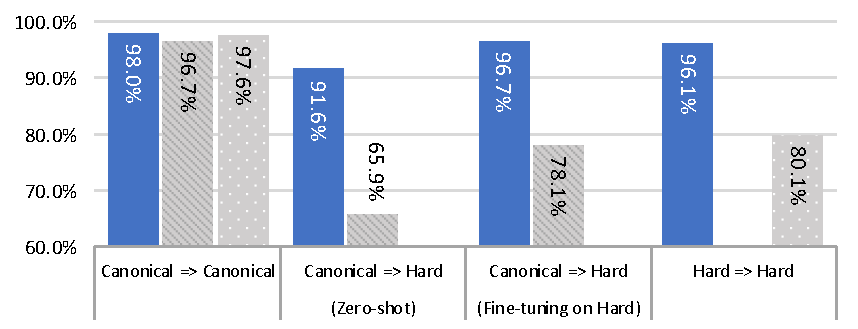
\includegraphics[width=\columnwidth]{../img/plots/cog_temporal_transfer_baselines.pdf}
	\caption{Total accuracies of SAMNet (blue) and baseline models (gray (dotted) / yellow (striped)) when testing generalization from Canonical to Hard variants of the dataset.}
	\label{fig:samnet_cog_overall_transfer}
\end{figure}


\subsection{Reasoning transfer in CoGenT}
\label{sec:reasoning-clevr}

\begin{figure}[htbp]
	\centering
	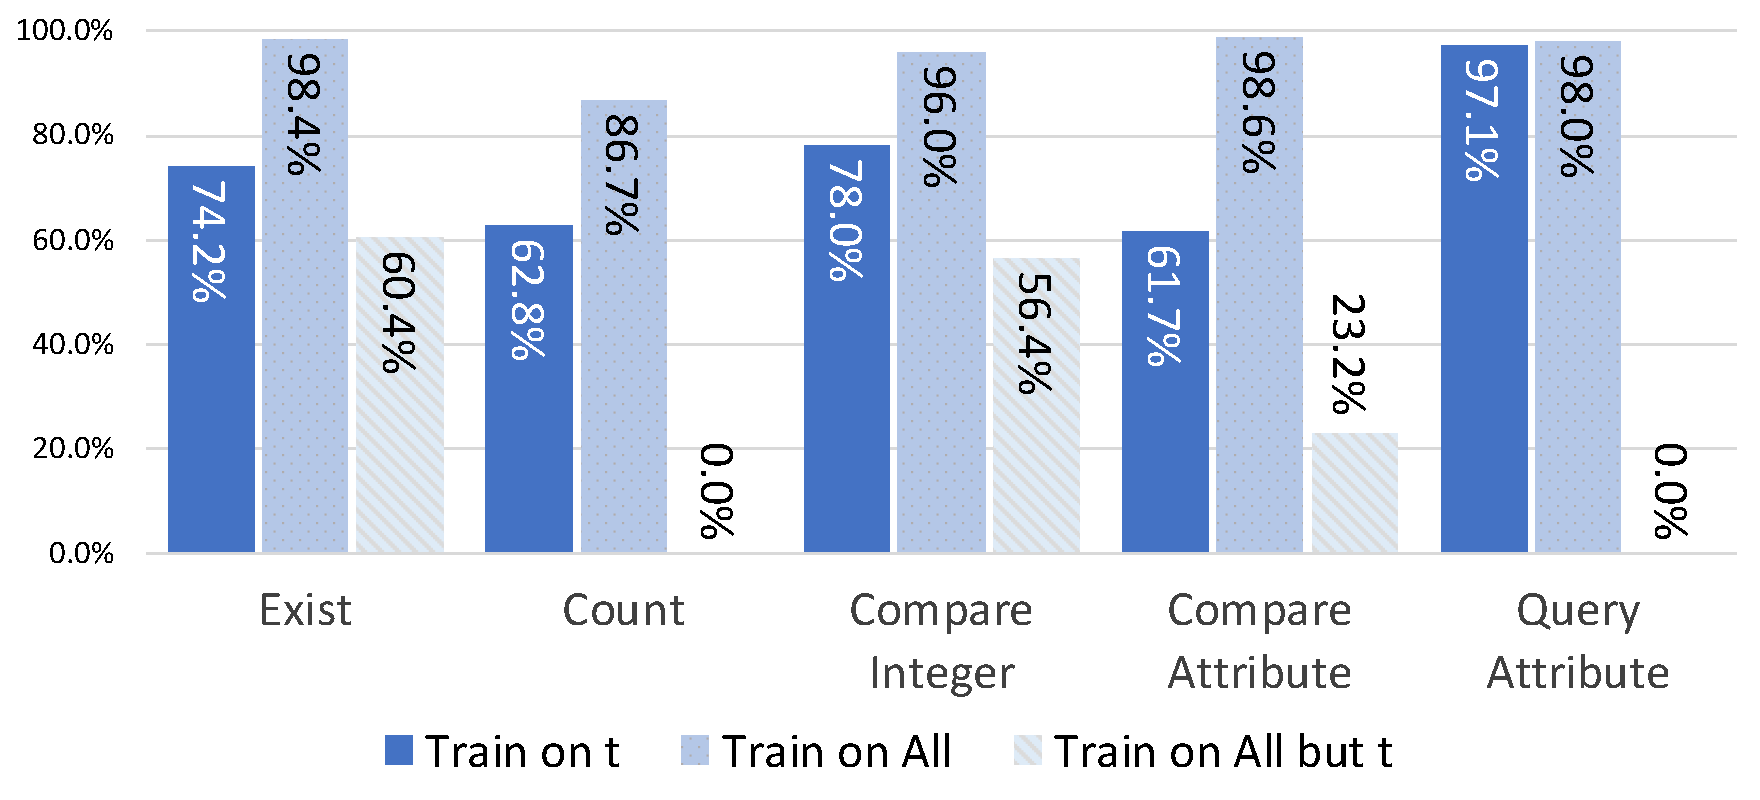
\includegraphics[width=\columnwidth]{../img/plots/cogent_reasoning_transfer.pdf}
	\caption{CoGenT-A accuracies for all tasks $t$ when training on $t$ only, training on all tasks jointly and training on all tasks but $t$.}
	\label{fig:CoGenT-results}
\end{figure}

Using the question categories defined by the author, we conduct the following experiments:
\begin{itemize}
	\compresslist
	\item Train and test SAMNet on a single task group $t$. These 5 experiments fit into the traditional ML setup of single-task learning;
	\item Train SAMNet on all task groups jointly and evaluate its performance on each task group $t$ separately.
	This is a transfer learning setting where for the source task family, the task is sampled from all questions, while for the target task family, the samples consist of questions from group $t$ only;
	\item Finally, for each task group $t$, we train SAMNet on all tasks but $t$, and test its performance on $t$. This can also be viewed as a transfer learning setting similar to the previous case.
\end{itemize}

Noticeable results are shown in~\cref{fig:CoGenT-results}, while the complete set is available in the supplementary material.

Looking at~\cref{fig:CoGenT-results}, SAMNet does well on \textit{Count} and \textit{QueryAttribute}, but poorer on the 3 other tasks in the single-task learning setting (blue). Indeed, \textit{Exist}, \textit{CompareInteger} and \textit{CompareAttribute} are binary tasks; \textit{Count} has output labels digits 0 through 10 (so $<$10\% accuracy by chance) and \textit{QueryAttribute} maps to the set of object-attribute values (15 labels).

Nevertheless, significant accuracy gains are noted when training jointly on all tasks (gray), ranging from 18 points to 37 points on 4 out of 5 tasks. These improvements suggest that related tasks benefit from joint training. \textit{QueryAttribute} only sees an increase of one point. One could qualify it as \textit{self-sufficient} as it does not appear to benefit from joint training with other tasks.

Finally, the ``all-tasks-but-$t$'' experiments (yellow) demonstrate that while tasks are related, one does not subsume another in terms of learning. Indeed, we can observe that for \textit{CompareAttribute}, while \textit{Exist} and \textit{CompareInteger} share the same output space, including them and holding out \textit{CompareAttribute} from the training set results in poor accuracy.
We also observe no learning for \textit{Count} and \textit{QueryAttribute}. As these categories have labels that do not overlap with other categories, the model cannot predict these labels.

An additional set of experiments, for which results are available in the supplementary material, fine-tune the model trained on all tasks on each task $t$ respectively.
Fine-tuning did not demonstrate a clear benefit (except for \textit{Count}, where the accuracy increased by 1.5 pt) without hurting performance on the other tasks. Nevertheless, these experiments leave open the possibility that joint training of tasks may potentially benefit from using weighted sampling towards the tail end with more emphasis on samples from less performing task groups, similar to~\cite{guo2018dynamic, kendall2018multi}.

\subsection{Reasoning transfer in COG}
\label{sec:reasoning-cog}

\begin{figure}[htbp]
	\centering
	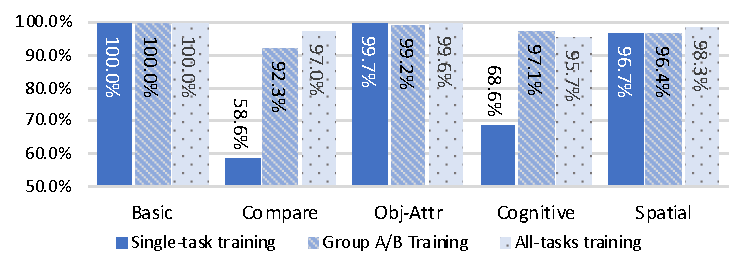
\includegraphics[width=\columnwidth]{../img/plots/cog_reasoning_transfer.pdf}
	\caption{COG accuracies for all task groups $t$ when training on $t$ only; training on Group A or B; and on all tasks.}
	\label{fig:COG-reasoning-results}
\end{figure}\vspace{2pt}

Reusing the task hierarchy in \cref{fig:task-groups}, we conduct the following experiments using the Canonical variant of COG to study whether transfer learning was effective in leveraging information gained by training a task family at a higher level
of the hierarchy:
 \begin{itemize}
 	\compresslist
	\item Train and test SAMNet on each of the 5 task groups at the lowest level of the hierarchy (Single-task training);
	\item Jointly train on:
	\begin{itemize}
		\item \textbf{Group A} and test on each task from the lowest groups (i.e. \textbf{Basic}, \textbf{Obj-Attr} and \textbf{Compare}) separately;
		\item \textbf{Group B} and test separately on \textbf{Spatial} and \textbf{Cognitive};
	\end{itemize}
	\item As a baseline, we compared the above results to the earlier experiment shown in~\cref{fig:samnet_cog_detailed}, which can be viewed as training jointly on \textbf{All} and testing on each group at the leaf level separately (All-task training).
\end{itemize}

The results of these experiments are shown in~\cref{fig:COG-reasoning-results}.

First, notice that for each of the \textbf{Basic} and \textbf{Obj-Attr} task families, the accuracy is near-perfect in all cases, suggesting that each contains the most primitive tasks and therefore do not benefit from training with other task families.
With \textbf{Spatial}, we see a small improvement showing that there is some benefit due to joint training with other task families.
Two groups that demonstrated a huge improvement of more than 25 points are \textbf{Compare} and \textbf{Cognitive}.
The former saw an accuracy jump from 58.6\% by training on samples from that family alone
to 97.0\% when training on all samples. To further emphasize this behavior, notice that
just joining \textbf{Compare} with \textbf{Obj-Attr} and \textbf{Basic} already causes a significant accuracy jump to 92.3\%.
In hindsight, this is not surprising, as the questions in \textbf{Compare} are composed
of fragments of questions given by \textbf{Basic} and \textbf{Obj-Attr}, and therefore can leverage the reasoning strategies developed there to reason about questions in \textbf{Compare}.
Lastly, for the \textbf{Spatial} family, we again see the benefits of joint training with all questions (68.6\% to 95.7\%) but in this case there
is a slight loss incurred by including everything. As seen in the figure, just jointly training with \textbf{Spatial} alone is sufficient to get a boost in accuracy (97.1\%). To summarize, while joint training helps, one needs to determine how much of correlation is present with the other tasks.
